%% -*- TeX-engine: luatex; ispell-dictionary: "english" -*-

\documentclass[unicode,11pt]{beamer}

\usepackage{algpseudocode}
\usepackage{tikz}
\usetikzlibrary{bayesnet}
\usetikzlibrary{arrows}

\PassOptionsToPackage{obeyspaces}{url}

\usetheme{Pittsburgh}
\usecolortheme{beaver}

\newenvironment{stopperenv}{\only{\setbeamercolor{local structure}{fg=darkred}}}{}

\setbeamercolor{frametitle}{fg=black,bg=white}
\setbeamerfont{frametitle}{size=\Large}
\setbeamertemplate{footline}[frame number]
\setbeamertemplate{frametitle continuation}{(\insertcontinuationcount)}
\setbeamertemplate{caption}{\insertcaption}
\setbeamertemplate{enumerate items}[default]
\setbeamertemplate{frametitle}{\hfill\insertframetitle\vskip-6pt\hrulefill}

\setbeamercovered{dynamic} % overlays not yet revealed will faintly appear
\beamertemplatenavigationsymbolsempty

\usepackage{fontspec}
\setmainfont{PT Serif}
\setsansfont{PT Sans}
\setmonofont[Ligatures=NoCommon]{PT Mono}
\defaultfontfeatures{Ligatures=TeX}

% sans serif for headings
\setbeamerfont*{block title}{family=\sffamily,series=\bfseries}

%\usepackage{microtype}


\newcommand{\theme}[1]{%
  \centering\fontsize{36pt}{1em}\color{darkred}{\selectfont{#1}}
}

\usepackage{polyglossia}
\setdefaultlanguage{english}
\usepackage{csquotes}

\usepackage[normalem]{ulem}

\usepackage{hyperref}
\hypersetup{
	colorlinks=true,
    linkcolor=darkred,
    urlcolor=darkred,
    citecolor=darkred
}

\makeatletter
\let\@mycite\@cite
\def\@cite#1#2{{\hypersetup{linkcolor=darkred}[{#1\if@tempswa , #2\fi}]}}
\makeatother

\usepackage{caption}
\captionsetup[figure]{labelformat=empty}

\usepackage{amsmath}
\usepackage{amssymb}
\DeclareMathOperator*{\argmin}{arg\,min}
\DeclareMathOperator*{\argmax}{arg\,max}

\newcommand{\op}[1]{\operatorname{#1}}


\title{Variational Auto-Encoder and normalizing flows}
\author{S. Lebedev, E. Tuzova}
\institute{JetBrains}
\date{\today}

%% Alternative title: variational auto-encoder + normalizing flows = ?

\begin{document}

% 1
\begin{frame}[plain,noframenumbering]
  \maketitle
\end{frame}


\begin{frame}{Motivation\footnote{Slide credit: G. Hinton, CSC2515, <<Continuous
      Latent Variable Models>>.}}
  \begin{center}
    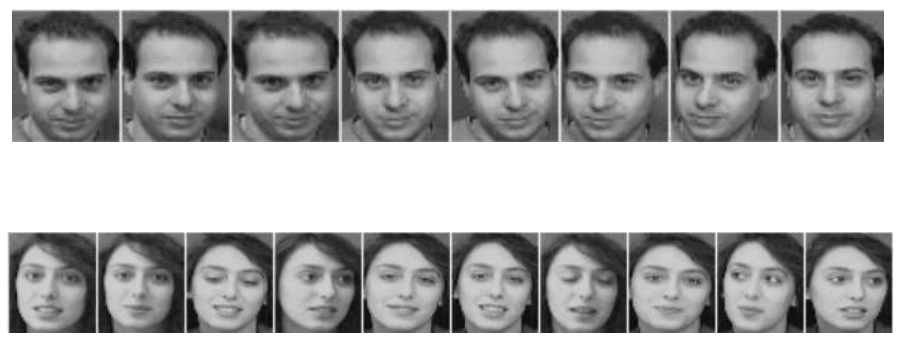
\includegraphics[width=.8\textwidth]{images/motivation}
  \end{center}

  \begin{itemize}
  \item What are the underlying latent dimensions in these two datasets?
  \item How do we find these from the data?
  \end{itemize}
\end{frame}

% 2
\begin{frame}[fragile]{Problem scenario}
  \begin{center}
    \begin{minipage}[t]{.3\linewidth}
      \begin{tikzpicture}[baseline=0]
        \node[latent]            (z) {$\mathbf{z}$};
        \node[obs, below=of z]   (x) {$\mathbf{x}$};
        \node[const, right=of z] (t) {$\theta$};
        \node[const, left=of x, xshift=2em]   (lfantom) {};
        \node[const, right=of x, xshift=-2em] (rfantom) {};

        \edge {z} {x};
        %\draw (x) edge [->,dashed,bend left=45] (z);
        \edge {t} {x,z};

        \plate {xz} {(x)(z)(lfantom)(rfantom)} {$~N$};
      \end{tikzpicture}
    \end{minipage}
    \begin{minipage}[t]{.55\linewidth}
      % $X = \left\{ x^{(i)}\right\}_{i=1}^N~-$ dataset\\
      $x$ --- observed variables\\
      $z$ --- \underline{continuous} latent variables\\
      $\theta$ --- model parameters\\
      % $\phi~-$ variational parameters\\
      $p_{\theta}(x, z) = p_{\theta}(x|z) p_{\theta}(z)$ --- joint p.d.f.\\
    \end{minipage}
  \end{center}

  \begin{itemize}
  \item Goal: fast approximate posterior inference for the latent variables
    in the ``real-world'' scenario.
  \item Specifically when
    \begin{itemize}
    \item evidence is \underline{intractable},
    \item so is the posterior for latent variables.
    \item Mean-field VB is \underline{not applicable} because the integrals
      required are intractable as well.
    \end{itemize}
  \end{itemize}

  %% TODO: scalable as well? or expand on fast.
\end{frame}


\begin{frame}{What are the options?}
  \begin{itemize}
  \item MCMC
    \begin{itemize}
    \item slow for large-scale problems,
    \item diagnosing convergence is an issue.
    \end{itemize}
  \item MAP
    \begin{itemize}
    \item easy to overfit the data,
    \item especially in the case of high-dimensional $z$.
    \end{itemize}
  \item VB
    \begin{itemize}
    \item mean-field cannot be applied directly,
    \item but still a good idea,
    \item maybe.
    \end{itemize}
  \end{itemize}
\end{frame}


\begin{frame}{The plan}
  \begin{enumerate}
  \item Approximate the posterior with a neural net
    $q_{\phi}(z|x)$, where $\phi$ --- variational parameters.
  \item Lower bound the evidence using $q_{\phi}(z|x)$.
  \item Construct an estimator of the ELBO which can be
    optimized jointly w.r.t. $\phi$ and $\theta$.
  \item Use stochastic gradient ascent.
  \item Profit.
  \end{enumerate}
\end{frame}


\begin{frame}{Encoder-decoder perspective}
  %% TODO
\end{frame}


\begin{frame}{ELBO}
  Having $q_\phi(z|x)$ we can deconstruct the evidence into
  $$
  \log p_\theta(x) = \KL{q_\phi(z|x)}{p_\theta(z|x)} + \mathcal{L}(\theta, \phi; x)
  $$
  where the lower bound is given by
  \begin{align*}
    \mathcal{L}(\theta, \phi; x)
    &= \E{q_\phi(z|x)}{\log p_\theta(x, z) - \log q_\phi(z|x)} \\
    &= -\KL{q_\phi (z|x)}{p_\theta(z)} + \E{q_\phi(z|x)}{\log p_\theta (x|z)}
  \end{align*}

  % \begin{itemize}
  %   \item $q(z|x)$ is not necessarily factorial
  %   \item Parameters $\phi$ are not computed from some closed-form expectation
  % \end{itemize}
\end{frame}


\begin{frame}{Optimizing the ELBO}
  \begin{itemize}
  \item Want to optimize the lower bound w.r.t both $\theta$ and $\phi$.
  \item Just-do-it approach:
    \begin{align*}
      \grad_\theta \mathcal{L}(\theta, \phi; x)
      &= \grad_\theta \E{q_\phi(z|x)}{\log p_\theta(x, z) - \log q_\phi(z|x)} \\
      &= \E{q_\phi(z|x)}{\grad_\theta \log p_\theta(x, z)} \\
      &\approx \frac{1}{S} \sum\limits_{s = 1}^S \grad_\theta \log p_\theta(x, z^{(s)}) \\
      \grad_\phi \mathcal{L}(\theta, \phi; x)
      &= \grad_\phi \E{q_\phi(z|x)}{\log p_\theta(x, z) - \log q_\phi(z|x)} \\
      &= -\grad_\phi \E{q_\phi(z|x)}{\log q_\phi(z|x)}
       = \op{:(}
    \end{align*}
  \item How to deal with the gradients of the form $\grad_\phi \E{q_\phi(z)}{f(z)}$?
  \end{itemize}
\end{frame}


\begin{frame}{Na\"ive MCMC estimator of $\grad_\phi \E{q_\phi(z)}{f(z)}$}
  \begin{align*}
    \grad_\phi \E{q_\phi(z)}{f(z)}
    &= \grad_\phi \int q_\phi(z) f(z) dz
     = \int f(z) \grad_\phi q_\phi(z) dz \\
    &= \int f(z) q_\phi(z) \grad_\phi \log q_\phi(z) dz
  \end{align*}
  where the last line is due to the log derivative
  trick\footnote{%
    \url{http://blog.shakirm.com/2015/11/machine-learning-trick-of-the-day-5-log-derivative-trick}}
  $$
  \grad_\phi \log q(z|x) = \frac{\grad_\phi q(z|x)}{q(z|x)}
  $$
  Proceeding further we obtain
  \begin{align*}
    \grad_\phi \E{q_\phi(z)}{f(z)}
    &= \E{q_\phi(z|x)}{f(z) \grad_\phi \log q_\phi(z)} \\
    &\approx \frac{1}{S} \sum\limits_{s = 1}^S f(z^{(s)}) \grad_\phi \log q_\phi(z^{(s)})
    \to \op{:(}
  \end{align*}

  %% TODO: covariance of sample mean is Cov(mean(X)) = Cov(X) / S,
  %% thus if the diagonal entries in Cov(X) are large, S must be
  %% large as well.
\end{frame}


\begin{frame}{Reparametrization trick%
  \footnote{\url{http://blog.shakirm.com/2015/10/machine-learning-trick-of-the-day-4-reparameterisation-tricks}}}
  \begin{itemize}
  \item Introduce an auxilary noise variable $\epsilon$ independent of $\phi$.
  \item Express $z$ as a determinisitic transformation of $\epsilon$
    differentiable w.r.t. $\phi$
    $$
    z = g_\phi(\epsilon, x)
    \qquad
    \epsilon \sim p(\epsilon)
    $$
  \item Plug the transformed variable into the expectation
    \begin{align*}
      \E{q_\phi(z|x)}{f(z)}
      = \E{p(\epsilon)}{f(g_\phi(\epsilon, x)}
      = \frac{1}{S} \sum\limits_{s = 1}^S f(g_\phi(\epsilon^{(l)}, x))
    \end{align*}
  \item A trivial but useful example:
    \begin{align*}
      q_\phi(z|x) = \mathcal{N}(z; \mu, \sigma^2)
      \qquad
      z = \mu + \sigma\epsilon
      \qquad
      \epsilon \sim \mathcal{N}(0, 1)
    \end{align*}
    \begin{align*}
      \grad_\phi \E{q_\phi(z)}{f_\theta(z)}
      = \E{\mathcal{N}(\epsilon; 0, 1)}{\grad_\phi f_\theta(\mu + \sigma \varepsilon)}
    \end{align*}
  \end{itemize}
\end{frame}


\begin{frame}[fragile]{SGVB estimator}
  \begin{align*}
    \mathcal{L}(\theta, \phi; x)
    &= \E{q_\phi(z|x)}{\log p_\theta(x, z) - \log q_\phi(z|x)} \\
    &\approx \frac{1}{S} \sum\limits_{s = 1}^S
          \log p_\theta(x, z^{(s)}) - \log q_\phi(z^{(s)}|x) \\
    &\doteq \tilde{\mathcal{L}}(\theta, \phi; x)
  \end{align*}
  where
  \begin{align*}
    z^{(s)} = g_\phi(\epsilon^{(s)}, x)
    \qquad
    \epsilon^{(s)} \sim p(\epsilon)
  \end{align*}
\end{frame}

%% TODO: the case of tractable KL? since we use it in experiments.

\begin{frame}{AEVB algorithm}
  \centering
  \begin{algorithmic}
    \State $\theta, \phi \gets$ initialize parameters
    \Repeat
       \State $X^M \gets$ random minibatch of $M$ datapoints
       \State $\epsilon \gets$ random samples from $p(\epsilon)$
       \State $g_\theta, g_\phi \gets \grad_{\phi, \theta} \mathcal{\tilde{L}}(\theta, \phi; X^M, \epsilon)$
       \State $\theta \gets \theta + \alpha g_\theta$
       \State $\phi \gets \phi + \alpha g_\phi$
    \Until convergence of parameters $\theta$, $\phi$ \\
    \Return $\theta$, $\phi$
  \end{algorithmic}
\end{frame}


\begin{frame}[fragile]{VAE inference model}
  \textcolor{darkred}{The VAE approach}: introduce an inference model that
  learns to approximate the intractable posterior by optimizing the variational lower bound:
  $$ \mathcal{L}(\theta, \phi, x) = -\mathbb{D}_{KL}[q_{\phi} (z|x) \parallel p(z)] +
  \mathbb{E}_q [\log p_\theta (x|z)] $$
  We parameterize with another neural network:
  \begin{figure}[htbp]
    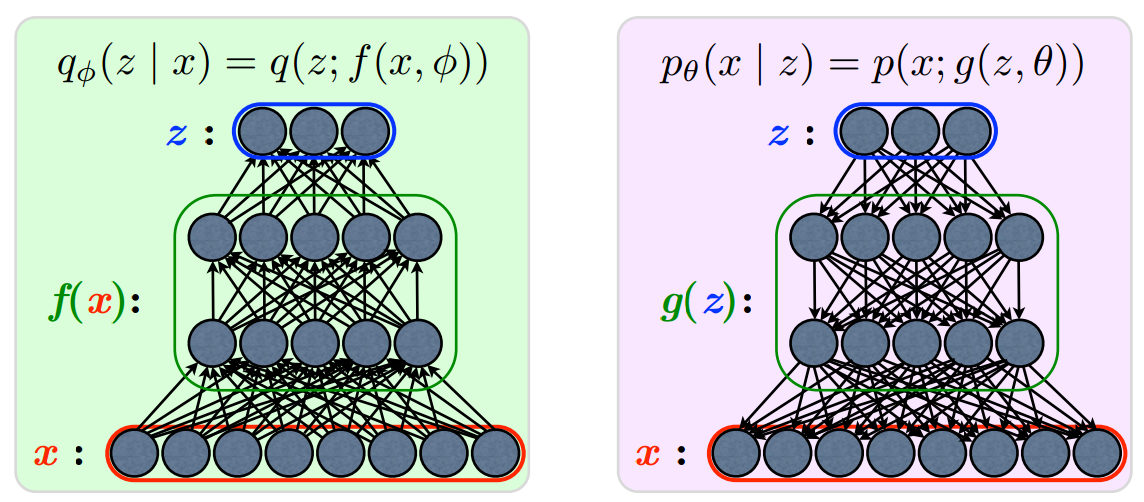
\includegraphics[height=130pt, keepaspectratio = true]{images/vae}
  \end{figure}
  \tiny \textcolor{gray}{http://videolectures.net/deeplearning2015\_courville\_autoencoder\_extension}
\end{frame}

% 13
\begin{frame}[fragile]{Coding theory perspective}
  The unobserved variables $z$ have an interpretation as a latent representation or code.

  \begin{itemize}
    \item Represent recognition model $q_{\phi}(z|x)$ as a probabilistic encoder.\\
        Given a datapoint $x$ it produces a distribution over the possible values of the code $z$
        from which the datapoint $x$ could have been generated
    \item Represent $p_{\theta}(x|z)$ as a probabilistic decoder.\\
        Given a code $z$ it produces a distribution over the possible corresponding values of $x$
  \end{itemize}
\end{frame}

% 14
\begin{frame}[fragile]{Variational Auto-Encoder}
  $p_{\theta}(z) = \mathcal{N}(z;0, I)$\\
  $p_{\theta}(x|z) ~-$ multivariate Gaussian, distribution parameters are computed from
  $z$ with a MLP\\
  $p_{\theta}(z|x) ~-$ intractable, takes on an approximate Gaussian form with an approximately diagonal covariance\\
  ~\\
  $q_{\phi}(z|x^{(i)}) = \log \mathcal{N}(z; \mu^{(i)}, \sigma^{2(i)} I) $\\
  $\mu^{(i)}, \sigma^{(i)} ~-$ outputs of the encoding MLP\\
  ~\\
  $L(\theta, \phi; x^{(i)}) \simeq \frac{1}{2} \sum\limits_{j=1}^J (1 + \log ((\sigma_j^{(i)})^2) -
  (\mu_j^{(i)})^2 - (\sigma_j^{(i)})^2) + \frac{1}{L} \sum\limits_{l=1}^L \log p_{\theta} (x^{(i)}|z^{(i,l)})$\\
  where $z^{(i,l)} = \mu^{(i)} + \sigma^{(i)} \odot \varepsilon^{(l)}$ and $\varepsilon^{(l)} \sim \mathcal{N}(0,I)$
\end{frame}

% 15
\begin{frame}[fragile]{Model restriction}
  How can we get closer to $p_{\theta}(z|x)$?
\end{frame}

% 16
\begin{frame}[fragile]{Normalizing flows}
  \textcolor{darkred}{Normalizing flows}: the transformation of a probability density through
  a sequence of invertible mappings.
  \begin{itemize}
    \item By repeated application of the rule for random variable transformations, the initial
    density flows through the sequence of invertible mappings.
    \item At the end of the sequence, we have a valid probability distribution.
  \end{itemize}

\end{frame}

% 17
\begin{frame}[fragile]{Normalizing flows}
  Transformation of random variables: $z' = f(z)$, $f^{-1}(z') = z$\\
  $$q(z') = q(z) \left\vert \det \frac{\partial f^{-1}(z')}{\partial z'} \right\vert =
  q(z) \left\vert \det \frac{\partial f(z')}{\partial z'} \right\vert^{-1}$$\\
  Chaining together a sequence: $z_K = f_K \circ f_{K−1} \circ \cdots \circ f_2 \circ f_1(z_0)$\\
  $$\log q_K(z_K) = \log q_0(z_0) − \sum_{k=1}^K \log \left\vert \det \frac{\partial f_k}{\partial z_k} \right\vert $$

  Law of the unconscious statistician:\\
  $$\mathbb{E}_{q_K} \left[g(z_K)\right] = \mathbb{E}_{q_0} \left[ g(f_K \circ f_{K−1} \circ \cdots \circ f_2
  \circ f_1(z_0)) \right] $$
\end{frame}

% 18
\begin{frame}[fragile]{Planar flow}
  \textcolor{darkred}{Family of transformations}: $f(z) = z + uh\left( w^T z + b \right)$\\
  ~\\
  $$\left\vert \det \frac{\partial f(z)}{\partial z} \right\vert = \left\vert 1 + u^T \psi(z)
  \right\vert ~~~\text{where}~~~ \psi(z) = h'(w^Tz + b)w$$ \\
  $$\log q_K(z_K) = \log q_0(z_0) − \sum_{k=1}^K \log \left\vert 1 + u^T \psi(z) \right\vert $$\\
  ~\\
  This flow modifies the initial density $q_0$ by applying a series of contractions and expansions in
  the direction perpendicular to the hyperplane $w^Tz+b = 0$.

  % TODO: картиночки (применение потока + обучение потока)
\end{frame}

% 19
\begin{frame}[fragile]{Radial flow}
  \textcolor{darkred}{Family of transformations}: \\
  $f(z) = z + \beta h(\alpha, r)(z-z_0) ~~~\text{where}~~~ r = \vert z-z_0 \vert$,
  $h(\alpha, r) = \frac{1}{\alpha + r}$\\
  ~\\
  $\det \left\vert \frac{\partial f}{\partial z} \right\vert = [1 + \beta h(\alpha, r)]^{(d-1)}
  [1 + \beta h(\alpha, r) + h'(\alpha, r) r]$\\
  ~\\
  This flow applies radial contractions and expansions around the reference point $z_0$.
\end{frame}

% 20
\begin{frame}[fragile]{Examples}
  TODO
  % картинка про поток?
\end{frame}

% 21
\begin{frame}[fragile]{Variational lower bound}
  \begin{align*}
  \mathcal{L}(\theta, \phi, x) &= \mathbb{E}_{q_\phi(z|x)} \left[ \log p_\theta(x, z) - \log q_\phi(z | x) \right] \\
  &= \mathbb{E}_{q_K(z_K)} \left[ \log p(x, z_K) - \log q(z_K) \right] \\
  &= \mathbb{E}_{q_0(z_0)} \left[ \log p(x, z_K) - \log q_0(z_0) + \sum_{k=1}^K \log \left\vert \det
  \frac{\partial f_k}  {\partial z_k} \right\vert \right]
  \end{align*}
\end{frame}

% 22
\begin{frame}[fragile]{Algorithm}
  \begin{algorithmic}
    \State $\theta, \phi \gets$ initialize parameters
    \Repeat
       \State $X^M \gets$ Random minibatch of $M$ datapoints
       \State $z_0 \sim q_0(\bullet|x)$
       \State $z_k \gets f_K \circ f_{K-1} \circ \cdots \circ f_1(z_0)$
       \State $L(x) \approx L(x, z_k)$
       \State $g \gets \nabla_{\phi, \theta} \mathcal{L}^M(\theta, \phi; X^M, \varepsilon) $ Gradients of minibatch estimator
       \State $\theta, \phi \gets$ Update parameters using gradients $g$
    \Until {convergence of parameters $\theta$, $\phi$}\\
    \Return $\theta$, $\phi$
  \end{algorithmic}

\end{frame}

% 23
\begin{frame}[fragile]{Algorithm}
  Normalizing flow integration into the VAE:\\
  \begin{figure}[htbp]
    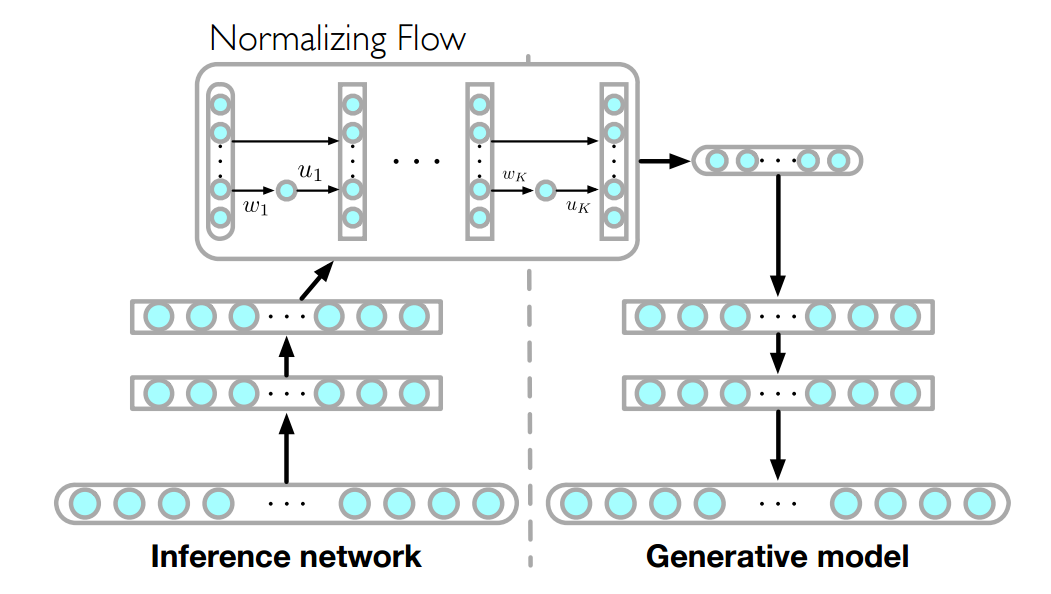
\includegraphics[height=130pt, keepaspectratio = true]{images/norFlow}
  \end{figure}
  ~\\
  \tiny \textcolor{gray}{http://arxiv.org/pdf/1505.05770v4.pdf}
\end{frame}

% 24
\begin{frame}[fragile]{MNIST (vae, vae+nf)}
  TODO
  %картинки
  % график ELBO
\end{frame}

% 25
\begin{frame}[fragile]{Frey Faces}
  TODO
  %картинки
\end{frame}

% 26
\begin{frame}[fragile]{Future experiments}
  TODO
\end{frame}

\end{document}
